\documentclass[twoside]{book}

% Packages required by doxygen
\usepackage{fixltx2e}
\usepackage{calc}
\usepackage{doxygen}
\usepackage[export]{adjustbox} % also loads graphicx
\usepackage{graphicx}
\usepackage[utf8]{inputenc}
\usepackage{makeidx}
\usepackage{multicol}
\usepackage{multirow}
\PassOptionsToPackage{warn}{textcomp}
\usepackage{textcomp}
\usepackage[nointegrals]{wasysym}
\usepackage[table]{xcolor}

% Font selection
\usepackage[T1]{fontenc}
\usepackage[scaled=.90]{helvet}
\usepackage{courier}
\usepackage{amssymb}
\usepackage{sectsty}
\renewcommand{\familydefault}{\sfdefault}
\allsectionsfont{%
  \fontseries{bc}\selectfont%
  \color{darkgray}%
}
\renewcommand{\DoxyLabelFont}{%
  \fontseries{bc}\selectfont%
  \color{darkgray}%
}
\newcommand{\+}{\discretionary{\mbox{\scriptsize$\hookleftarrow$}}{}{}}

% Page & text layout
\usepackage{geometry}
\geometry{%
  a4paper,%
  top=2.5cm,%
  bottom=2.5cm,%
  left=2.5cm,%
  right=2.5cm%
}
\tolerance=750
\hfuzz=15pt
\hbadness=750
\setlength{\emergencystretch}{15pt}
\setlength{\parindent}{0cm}
\setlength{\parskip}{3ex plus 2ex minus 2ex}
\makeatletter
\renewcommand{\paragraph}{%
  \@startsection{paragraph}{4}{0ex}{-1.0ex}{1.0ex}{%
    \normalfont\normalsize\bfseries\SS@parafont%
  }%
}
\renewcommand{\subparagraph}{%
  \@startsection{subparagraph}{5}{0ex}{-1.0ex}{1.0ex}{%
    \normalfont\normalsize\bfseries\SS@subparafont%
  }%
}
\makeatother

% Headers & footers
\usepackage{fancyhdr}
\pagestyle{fancyplain}
\fancyhead[LE]{\fancyplain{}{\bfseries\thepage}}
\fancyhead[CE]{\fancyplain{}{}}
\fancyhead[RE]{\fancyplain{}{\bfseries\leftmark}}
\fancyhead[LO]{\fancyplain{}{\bfseries\rightmark}}
\fancyhead[CO]{\fancyplain{}{}}
\fancyhead[RO]{\fancyplain{}{\bfseries\thepage}}
\fancyfoot[LE]{\fancyplain{}{}}
\fancyfoot[CE]{\fancyplain{}{}}
\fancyfoot[RE]{\fancyplain{}{\bfseries\scriptsize Generated by Doxygen }}
\fancyfoot[LO]{\fancyplain{}{\bfseries\scriptsize Generated by Doxygen }}
\fancyfoot[CO]{\fancyplain{}{}}
\fancyfoot[RO]{\fancyplain{}{}}
\renewcommand{\footrulewidth}{0.4pt}
\renewcommand{\chaptermark}[1]{%
  \markboth{#1}{}%
}
\renewcommand{\sectionmark}[1]{%
  \markright{\thesection\ #1}%
}

% Indices & bibliography
\usepackage{natbib}
\usepackage[titles]{tocloft}
\setcounter{tocdepth}{3}
\setcounter{secnumdepth}{5}
\makeindex

% Hyperlinks (required, but should be loaded last)
\usepackage{ifpdf}
\ifpdf
  \usepackage[pdftex,pagebackref=true]{hyperref}
\else
  \usepackage[ps2pdf,pagebackref=true]{hyperref}
\fi
\hypersetup{%
  colorlinks=true,%
  linkcolor=blue,%
  citecolor=blue,%
  unicode%
}

% Custom commands
\newcommand{\clearemptydoublepage}{%
  \newpage{\pagestyle{empty}\cleardoublepage}%
}

\usepackage{caption}
\captionsetup{labelsep=space,justification=centering,font={bf},singlelinecheck=off,skip=4pt,position=top}

%===== C O N T E N T S =====

\begin{document}

% Titlepage & ToC
\hypersetup{pageanchor=false,
             bookmarksnumbered=true,
             pdfencoding=unicode
            }
\pagenumbering{alph}
\begin{titlepage}
\vspace*{7cm}
\begin{center}%
{\Large I\+GV \\[1ex]\large 1.\+2 }\\
\vspace*{1cm}
{\large Generated by Doxygen 1.8.13}\\
\end{center}
\end{titlepage}
\clearemptydoublepage
\pagenumbering{roman}
\tableofcontents
\clearemptydoublepage
\pagenumbering{arabic}
\hypersetup{pageanchor=true}

%--- Begin generated contents ---
\chapter{File Index}
\section{File List}
Here is a list of all files with brief descriptions\+:\begin{DoxyCompactList}
\item\contentsline{section}{/home/soobin/\+Documents/\+Sandbox/\+I\+G\+V/src/\hyperlink{BasicNavigation_8cpp}{Basic\+Navigation.\+cpp} }{\pageref{BasicNavigation_8cpp}}{}
\item\contentsline{section}{/home/soobin/\+Documents/\+Sandbox/\+I\+G\+V/src/\hyperlink{Camera_8cpp}{Camera.\+cpp} }{\pageref{Camera_8cpp}}{}
\item\contentsline{section}{/home/soobin/\+Documents/\+Sandbox/\+I\+G\+V/src/\hyperlink{GPS_8cpp}{G\+P\+S.\+cpp} }{\pageref{GPS_8cpp}}{}
\item\contentsline{section}{/home/soobin/\+Documents/\+Sandbox/\+I\+G\+V/src/\hyperlink{IGV_8cpp}{I\+G\+V.\+cpp} }{\pageref{IGV_8cpp}}{}
\item\contentsline{section}{/home/soobin/\+Documents/\+Sandbox/\+I\+G\+V/src/\hyperlink{LaneDetection_8cpp}{Lane\+Detection.\+cpp} }{\pageref{LaneDetection_8cpp}}{}
\item\contentsline{section}{/home/soobin/\+Documents/\+Sandbox/\+I\+G\+V/src/\hyperlink{LIDAR_8cpp}{L\+I\+D\+A\+R.\+cpp} }{\pageref{LIDAR_8cpp}}{}
\item\contentsline{section}{/home/soobin/\+Documents/\+Sandbox/\+I\+G\+V/src/\hyperlink{main_8cpp}{main.\+cpp} }{\pageref{main_8cpp}}{}
\item\contentsline{section}{/home/soobin/\+Documents/\+Sandbox/\+I\+G\+V/src/\hyperlink{ObjectDetection_8cpp}{Object\+Detection.\+cpp} }{\pageref{ObjectDetection_8cpp}}{}
\item\contentsline{section}{/home/soobin/\+Documents/\+Sandbox/\+I\+G\+V/src/\hyperlink{Sensors_8cpp}{Sensors.\+cpp} }{\pageref{Sensors_8cpp}}{}
\item\contentsline{section}{/home/soobin/\+Documents/\+Sandbox/\+I\+G\+V/test/\hyperlink{test_8cpp}{test.\+cpp} }{\pageref{test_8cpp}}{}
\end{DoxyCompactList}

\chapter{File Documentation}
\hypertarget{BasicNavigation_8cpp}{}\section{/home/soobin/\+Documents/\+Sandbox/\+I\+G\+V/src/\+Basic\+Navigation.cpp File Reference}
\label{BasicNavigation_8cpp}\index{/home/soobin/\+Documents/\+Sandbox/\+I\+G\+V/src/\+Basic\+Navigation.\+cpp@{/home/soobin/\+Documents/\+Sandbox/\+I\+G\+V/src/\+Basic\+Navigation.\+cpp}}
{\ttfamily \#include \char`\"{}Basic\+Navigation.\+hpp\char`\"{}}\newline

\hypertarget{BasicNavigation_8cpp_source}{}\section{Basic\+Navigation.\+cpp}
\label{BasicNavigation_8cpp_source}\index{/home/soobin/\+Documents/\+Sandbox/\+I\+G\+V/src/\+Basic\+Navigation.\+cpp@{/home/soobin/\+Documents/\+Sandbox/\+I\+G\+V/src/\+Basic\+Navigation.\+cpp}}

\begin{DoxyCode}
00001 \textcolor{preprocessor}{#}\textcolor{preprocessor}{include} \textcolor{preprocessor}{"BasicNavigation.hpp"}
00002 
00003 \textcolor{keyword}{using} \textcolor{keyword}{namespace} igv;
00004 \textcolor{keyword}{using} \textcolor{keyword}{namespace} std;
00005 \textcolor{keyword}{using} \textcolor{keyword}{namespace} chrono;
00006 
00007 \textcolor{comment}{/*!}
00008 \textcolor{comment}{  * @brief Set the Speed of both motors}
00009 \textcolor{comment}{  * @param speed The Speed to set it to [-127, 127]}
00010 \textcolor{comment}{  */}
00011 \textcolor{keywordtype}{void} MotorController::SetSpeed(Speed speed)\{
00012 
00013   SetSpeed(LEFT, speed);
00014   SetSpeed(RIGHT, speed);
00015 
00016 \}
00017 
00018 \textcolor{preprocessor}{#}\textcolor{preprocessor}{ifndef} \textcolor{preprocessor}{SIMULATION}
00019 
00020 \textcolor{comment}{/*!}
00021 \textcolor{comment}{  * @brief Creates A Motor Controller Object}
00022 \textcolor{comment}{*/}
00023 MotorController::MotorController() : myport(MCPORT, B9600)\{
00024   busy = \textcolor{keyword}{false};
00025   speed = 0;
00026   direction = 0;
00027 \}
00028 
00029 \textcolor{comment}{/*!}
00030 \textcolor{comment}{  * @brief Sets the Speed of a motor}
00031 \textcolor{comment}{  * }
00032 \textcolor{comment}{  * @param motor The Motor to Set the Speed of}
00033 \textcolor{comment}{  * @param speed The Speed to Set it to}
00034 \textcolor{comment}{*/}
00035 \textcolor{keywordtype}{void} MotorController::SetSpeed(Motor motor, Speed speed) \{
00036 
00037   uint8\_t command = 0;
00038   string msg = \textcolor{stringliteral}{" "};
00039   uint8\_t magnitude = abs(speed) >> 1;
00040 
00041   \textcolor{keywordflow}{if} (motor == LEFT)
00042     command = speed < 0 ? 63 - magnitude : 64 + magnitude;
00043 
00044   \textcolor{keywordflow}{else}
00045     command = speed < 0 ? 191 - magnitude : 192 + magnitude;
00046 
00047   command = (!command)? 1: (command == 0xff)? 254: command;
00048 
00049   msg[0] = command;
00050 
00051   \textcolor{keyword}{this}->myport.Write(msg);
00052 
00053 \}
00054 
00055 \textcolor{comment}{/*!}
00056 \textcolor{comment}{  *  @brief Completes a turn while moving }
00057 \textcolor{comment}{  * }
00058 \textcolor{comment}{  *  @param deltadir Change in direction, [0, 2pi] -> [0, 256]}
00059 \textcolor{comment}{  *  @param speeddiff How much to take off of the motor speed [0, 127]}
00060 \textcolor{comment}{  * }
00061 \textcolor{comment}{  *  !The slower the speed and faster the speeddiff the faster and less wide the}
00062 \textcolor{comment}{  *  !turn}
00063 \textcolor{comment}{  */}
00064 
00065 \textcolor{keywordtype}{void} MotorController::ChangeDirection(DeltaDir deltadir, Speed speeddiff) \{
00066 
00067   \textcolor{keywordflow}{if} (busy || !deltadir || !speeddiff) \textcolor{keywordflow}{return}; \textcolor{comment}{// if busy or with bad params exit}
00068 
00069   \textcolor{keywordtype}{double} ohmega; \textcolor{comment}{// angular velocity in terms of change in direction per second}
00070                  \textcolor{comment}{// using dir: 0 = 0, 256 = 2pi}
00071   milliseconds waittime; \textcolor{comment}{// wait time to travel dir angular distance}
00072 
00073   direction += deltadir; \textcolor{comment}{// update the direction }
00074 
00075   speed &= 0x7f; \textcolor{comment}{// make sure the value is seven bits}
00076 
00077   \textcolor{keywordflow}{if} (((\textcolor{keywordtype}{int})speeddiff + \textcolor{keyword}{this}->speed) > 127)
00078     speeddiff = 127 - \textcolor{keyword}{this}->speed; \textcolor{comment}{// correct the speed diff if too high or low}
00079 
00080   \textcolor{keywordflow}{if} (((\textcolor{keywordtype}{int})\textcolor{keyword}{this}->speed - speeddiff) < -127)
00081     speeddiff = \textcolor{keyword}{this}->speed - 127;
00082 
00083   ohmega = ((\textcolor{keywordtype}{int})speeddiff << 7) / (PI * WHEELBASE); \textcolor{comment}{// get tangential speed and convert it to angular}
00084 
00085   waittime = milliseconds((uint64\_t)(1000 * abs(deltadir) / ohmega)); \textcolor{comment}{// calculate wait time in millis}
00086 
00087   busy = \textcolor{keyword}{true};
00088 
00089   SetSpeed(LEFT, deltadir > 0 ? \textcolor{keyword}{this}->speed - speeddiff
00090                               : \textcolor{keyword}{this}->speed + speeddiff); \textcolor{comment}{// give the motors their new speeds}
00091 
00092   SetSpeed(RIGHT, deltadir > 0 ? \textcolor{keyword}{this}->speed + speeddiff
00093                                : \textcolor{keyword}{this}->speed - speeddiff);
00094 
00095   this\_thread::sleep\_for(waittime); \textcolor{comment}{// wait until the turn has covered the delta}
00096 
00097   SetSpeed(\textcolor{keyword}{this}->speed); \textcolor{comment}{// go back to going straight}
00098 
00099   busy = \textcolor{keyword}{false};
00100 
00101 \}
00102 
00103 \textcolor{preprocessor}{#}\textcolor{preprocessor}{endif}
\end{DoxyCode}

\hypertarget{Camera_8cpp}{}\section{/home/soobin/\+Documents/\+Sandbox/\+I\+G\+V/src/\+Camera.cpp File Reference}
\label{Camera_8cpp}\index{/home/soobin/\+Documents/\+Sandbox/\+I\+G\+V/src/\+Camera.\+cpp@{/home/soobin/\+Documents/\+Sandbox/\+I\+G\+V/src/\+Camera.\+cpp}}
{\ttfamily \#include \char`\"{}Camera.\+hpp\char`\"{}}\newline
Include dependency graph for Camera.\+cpp\+:
\nopagebreak
\begin{figure}[H]
\begin{center}
\leavevmode
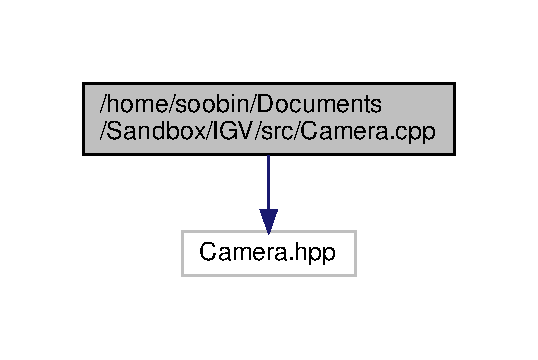
\includegraphics[width=258pt]{Camera_8cpp__incl}
\end{center}
\end{figure}

\hypertarget{Camera_8cpp_source}{}\section{Camera.\+cpp}
\label{Camera_8cpp_source}\index{/home/soobin/\+Documents/\+Sandbox/\+I\+G\+V/src/\+Camera.\+cpp@{/home/soobin/\+Documents/\+Sandbox/\+I\+G\+V/src/\+Camera.\+cpp}}

\begin{DoxyCode}
00001 
00002 \textcolor{preprocessor}{#}\textcolor{preprocessor}{include} \textcolor{preprocessor}{"Camera.hpp"}
00003 \textcolor{preprocessor}{#}\textcolor{preprocessor}{ifndef} \textcolor{preprocessor}{SIMULATION}
00004 
00005 \textcolor{keyword}{using} \textcolor{keyword}{namespace} igv;
00006 
00007 Camera::Camera(\textcolor{keywordtype}{int} port): cap(port) \{\}
00008 
00009 \textcolor{keywordtype}{void} Camera::Capture() \{ cap >> \textcolor{keyword}{this}->Image; \}
00010 
00011 \textcolor{preprocessor}{#}\textcolor{preprocessor}{else}
00012 
00013 \textcolor{preprocessor}{#}\textcolor{preprocessor}{endif}
\end{DoxyCode}

\hypertarget{GPS_8cpp}{}\section{/home/soobin/\+Documents/\+Sandbox/\+I\+G\+V/src/\+G\+PS.cpp File Reference}
\label{GPS_8cpp}\index{/home/soobin/\+Documents/\+Sandbox/\+I\+G\+V/src/\+G\+P\+S.\+cpp@{/home/soobin/\+Documents/\+Sandbox/\+I\+G\+V/src/\+G\+P\+S.\+cpp}}
{\ttfamily \#include \char`\"{}G\+P\+S.\+hpp\char`\"{}}\newline
Include dependency graph for G\+P\+S.\+cpp\+:
\nopagebreak
\begin{figure}[H]
\begin{center}
\leavevmode
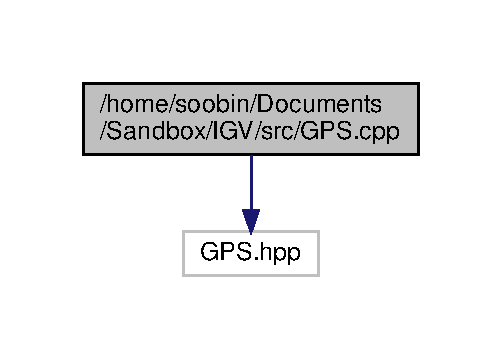
\includegraphics[width=241pt]{GPS_8cpp__incl}
\end{center}
\end{figure}

\hypertarget{GPS_8cpp_source}{}\section{G\+P\+S.\+cpp}
\label{GPS_8cpp_source}\index{/home/soobin/\+Documents/\+Sandbox/\+I\+G\+V/src/\+G\+P\+S.\+cpp@{/home/soobin/\+Documents/\+Sandbox/\+I\+G\+V/src/\+G\+P\+S.\+cpp}}

\begin{DoxyCode}
00001 \textcolor{preprocessor}{#}\textcolor{preprocessor}{include} \textcolor{preprocessor}{"GPS.hpp"}
00002 
00003 \textcolor{preprocessor}{#}\textcolor{preprocessor}{ifndef} \textcolor{preprocessor}{SIMULATION}
00004 \textcolor{keyword}{using} \textcolor{keyword}{namespace} mn::CppLinuxSerial;
00005 \textcolor{keyword}{using} \textcolor{keyword}{namespace} igv;
00006 
00007 GPS::GPS(): myport(GPSPORT, B9600)\{\}
00008 
00009 \textcolor{keywordtype}{void} GPS::Probe()\{
00010 
00011 \}
00012 
00013 Direction GPS::GetBearingTo(\textcolor{keywordtype}{double} lat, \textcolor{keywordtype}{double} lon)\{
00014     \textcolor{keywordflow}{return} \textcolor{keyword}{this}->gps.courseTo(\textcolor{keyword}{this}->CurrLat, \textcolor{keyword}{this}->CurrLong, lat, lon);
00015 \}
00016 
00017 \textcolor{keywordtype}{double} GPS::GetDistanceTo(\textcolor{keywordtype}{double} lat, \textcolor{keywordtype}{double} lon)\{
00018     \textcolor{keywordflow}{return} \textcolor{keyword}{this}->gps.distanceBetween(\textcolor{keyword}{this}->CurrLat, \textcolor{keyword}{this}->CurrLong,lat,lon);
00019 \}
00020 
00021 \textcolor{preprocessor}{#}\textcolor{preprocessor}{else}
00022 
00023 
00024 \textcolor{preprocessor}{#}\textcolor{preprocessor}{endif}
\end{DoxyCode}

\hypertarget{IGV_8cpp}{}\section{/home/soobin/\+Documents/\+Sandbox/\+I\+G\+V/src/\+I\+GV.cpp File Reference}
\label{IGV_8cpp}\index{/home/soobin/\+Documents/\+Sandbox/\+I\+G\+V/src/\+I\+G\+V.\+cpp@{/home/soobin/\+Documents/\+Sandbox/\+I\+G\+V/src/\+I\+G\+V.\+cpp}}
{\ttfamily \#include \char`\"{}I\+G\+V.\+hpp\char`\"{}}\newline
Include dependency graph for I\+G\+V.\+cpp\+:
\nopagebreak
\begin{figure}[H]
\begin{center}
\leavevmode
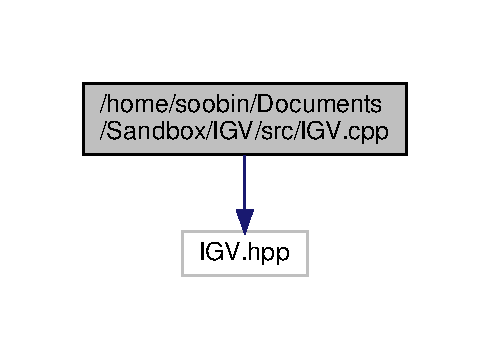
\includegraphics[width=235pt]{IGV_8cpp__incl}
\end{center}
\end{figure}

\hypertarget{IGV_8cpp_source}{}\section{I\+G\+V.\+cpp}
\label{IGV_8cpp_source}\index{/home/soobin/\+Documents/\+Sandbox/\+I\+G\+V/src/\+I\+G\+V.\+cpp@{/home/soobin/\+Documents/\+Sandbox/\+I\+G\+V/src/\+I\+G\+V.\+cpp}}

\begin{DoxyCode}
00001 
00002 \textcolor{preprocessor}{#}\textcolor{preprocessor}{include} \textcolor{preprocessor}{"IGV.hpp"}
00003 
00004 \textcolor{keyword}{using} \textcolor{keyword}{namespace} igv;
00005 \textcolor{keyword}{using} \textcolor{keyword}{namespace} chrono;
00006 
00007 \textcolor{preprocessor}{#}\textcolor{preprocessor}{ifndef} \textcolor{preprocessor}{SIMULATION}
00008 IGV::IGV() : LCam(LANECAMPORT), OCam(OBJCAMPORT)\{\}
00009 
00010 \textcolor{preprocessor}{#}\textcolor{preprocessor}{else}
00011 
00012 \textcolor{preprocessor}{#}\textcolor{preprocessor}{endif}
00013 
00014 \textcolor{keywordtype}{void} IGV::Setup()\{ \textcolor{comment}{// setup the threads }
00015 
00016   thread od(ObjDetection, \textcolor{keyword}{this});
00017   thread ld(LaneDetection, \textcolor{keyword}{this});
00018   thread sens(SensorLoop, \textcolor{keyword}{this});
00019   thread lid(LidarLoop, \textcolor{keyword}{this});
00020   thread gpsl(GPSLoop, \textcolor{keyword}{this});
00021 
00022   ld.join();
00023   od.join();
00024   sens.join();
00025   lid.join();
00026   gpsl.join();
00027 
00028 \}
00029 
00030 \textcolor{keywordtype}{void} IGV::Run()
00031 \{
00032 
00033   \textcolor{comment}{// TODO: Implemetation}
00034 \}
00035 
00036 \textcolor{keywordtype}{void} igv::ObjDetection(IGV* igv)\{
00037 
00038   igv->OCam.Capture();
00039   igv->OD.DetectObjects(igv->OCam.GetImage());
00040 
00041 \}
00042 
00043 \textcolor{keywordtype}{void} igv::LaneDetection(IGV* igv)\{
00044 
00045   igv->LCam.Capture();
00046   igv->LD.DetectLanes(igv->LCam.GetImage());
00047 
00048 \}
00049 
00050 \textcolor{keywordtype}{void} igv::LidarLoop(IGV* igv) \{
00051 
00052   igv->lidar.Probe();
00053 
00054 \}
00055 
00056 \textcolor{keywordtype}{void} igv::GPSLoop(IGV* igv)\{
00057 
00058   igv->gps.Probe();
00059 
00060 \}
00061 
00062 \textcolor{keywordtype}{void} igv::SensorLoop(IGV* igv)\{
00063 
00064   igv->us.Probe();
00065 
00066 \}
\end{DoxyCode}

\hypertarget{LaneDetection_8cpp}{}\section{/home/soobin/\+Documents/\+Sandbox/\+I\+G\+V/src/\+Lane\+Detection.cpp File Reference}
\label{LaneDetection_8cpp}\index{/home/soobin/\+Documents/\+Sandbox/\+I\+G\+V/src/\+Lane\+Detection.\+cpp@{/home/soobin/\+Documents/\+Sandbox/\+I\+G\+V/src/\+Lane\+Detection.\+cpp}}
{\ttfamily \#include \char`\"{}Lane\+Detection.\+hpp\char`\"{}}\newline
Include dependency graph for Lane\+Detection.\+cpp\+:
\nopagebreak
\begin{figure}[H]
\begin{center}
\leavevmode
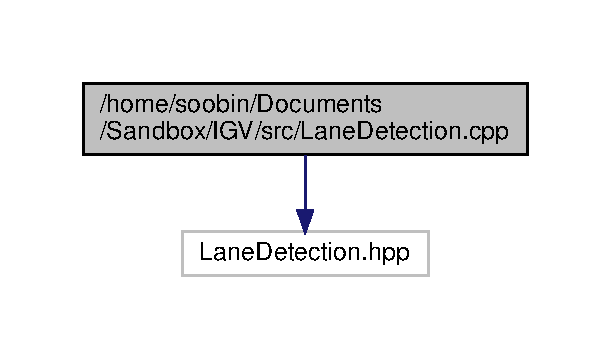
\includegraphics[width=293pt]{LaneDetection_8cpp__incl}
\end{center}
\end{figure}
\subsection*{Variables}
\begin{DoxyCompactItemize}
\item 
this \hyperlink{LaneDetection_8cpp_a9a499e6ee417732a06f9d3a3f6433546}{numlanes} = lines\+P.\+size()
\item 
\hyperlink{LaneDetection_8cpp_ab5707289495a33e90ac7ce232adcca4c}{busy} = false
\end{DoxyCompactItemize}


\subsection{Variable Documentation}
\mbox{\Hypertarget{LaneDetection_8cpp_ab5707289495a33e90ac7ce232adcca4c}\label{LaneDetection_8cpp_ab5707289495a33e90ac7ce232adcca4c}} 
\index{Lane\+Detection.\+cpp@{Lane\+Detection.\+cpp}!busy@{busy}}
\index{busy@{busy}!Lane\+Detection.\+cpp@{Lane\+Detection.\+cpp}}
\subsubsection{\texorpdfstring{busy}{busy}}
{\footnotesize\ttfamily busy = false}



Definition at line \hyperlink{LaneDetection_8cpp_source_l00258}{258} of file \hyperlink{LaneDetection_8cpp_source}{Lane\+Detection.\+cpp}.

\mbox{\Hypertarget{LaneDetection_8cpp_a9a499e6ee417732a06f9d3a3f6433546}\label{LaneDetection_8cpp_a9a499e6ee417732a06f9d3a3f6433546}} 
\index{Lane\+Detection.\+cpp@{Lane\+Detection.\+cpp}!numlanes@{numlanes}}
\index{numlanes@{numlanes}!Lane\+Detection.\+cpp@{Lane\+Detection.\+cpp}}
\subsubsection{\texorpdfstring{numlanes}{numlanes}}
{\footnotesize\ttfamily this numlanes = lines\+P.\+size()}



Definition at line \hyperlink{LaneDetection_8cpp_source_l00257}{257} of file \hyperlink{LaneDetection_8cpp_source}{Lane\+Detection.\+cpp}.


\hypertarget{LaneDetection_8cpp_source}{}\section{Lane\+Detection.\+cpp}
\label{LaneDetection_8cpp_source}\index{/home/soobin/\+Documents/\+Sandbox/\+I\+G\+V/src/\+Lane\+Detection.\+cpp@{/home/soobin/\+Documents/\+Sandbox/\+I\+G\+V/src/\+Lane\+Detection.\+cpp}}

\begin{DoxyCode}
00001 \textcolor{preprocessor}{#}\textcolor{preprocessor}{include} \textcolor{preprocessor}{"LaneDetection.hpp"}
00002 
00003 \textcolor{keyword}{using} \textcolor{keyword}{namespace} igv;
00004 \textcolor{keyword}{using} \textcolor{keyword}{namespace} std;
00005 \textcolor{keyword}{using} \textcolor{keyword}{namespace} cv;
00006 
00007 \textcolor{comment}{// Stream operator overload, allows you to print Lanes}
00008 ostream& igv::operator<<(ostream& os, Lane& lane)\{
00009 
00010     os << \textcolor{stringliteral}{"Lane Slope: "} << lane.slope << endl;
00011     os << (lane.slope == 0.0f? \textcolor{stringliteral}{" Y-Intercept: "} : \textcolor{stringliteral}{" X-Intercept: "});
00012     os << lane.intercept << endl;
00013 
00014     \textcolor{keywordflow}{return} os;
00015 \}
00016 
00017 \textcolor{preprocessor}{#}\textcolor{preprocessor}{ifndef} \textcolor{preprocessor}{\_\_NVCC\_\_}   \textcolor{comment}{// if not using the GPU}
00018 
00019 \textcolor{comment}{/* Lane Detection Function:}
00020 \textcolor{comment}{ * }
00021 \textcolor{comment}{ * Reads an image and finds the largest Lanes and fills an array with the 4 largest}
00022 \textcolor{comment}{ * @param: LaneArray: a preexisting array full of lanes that gets modified by the function}
00023 \textcolor{comment}{ * @param: image: a preexisting matrix representing an image that gets read for lanes}
00024 \textcolor{comment}{ * @retval: returns the number of lanes detected total}
00025 \textcolor{comment}{ * }
00026 \textcolor{comment}{ */}
00027 
00028 uint32\_t LaneDetector::DetectLanes(array<Lane, 4>& LaneArray, Mat& image)\{
00029 
00030     \textcolor{preprocessor}{#}\textcolor{preprocessor}{ifdef} \textcolor{preprocessor}{DEBUG}
00031     Mat imgcopy;
00032     image.copyTo(imgcopy);
00033     \textcolor{preprocessor}{#}\textcolor{preprocessor}{endif}
00034 
00035     Mat gray, edged;
00036     cvtColor(image, gray, COLOR\_BGR2GRAY);
00037     Canny(gray, edged, 200, 200 );
00038 
00039     vector<Vec4i> linesP;  \textcolor{comment}{// a vector to fill with line points}
00040     HoughLinesP(edged, linesP, 1, CV\_PI/256, 80, 80, 10);  \textcolor{comment}{// find the lines}
00041 
00042     \textcolor{keywordflow}{if}(linesP.size() < 1) \textcolor{keywordflow}{return} 0; \textcolor{comment}{// if there is less than one line return 0 lanes}
00043 
00044     \textcolor{comment}{// store index and magnitiude of largest lines and a temporary magnitude}
00045     \textcolor{keyword}{struct} linedata\{
00046 
00047       \textcolor{keywordtype}{double} mag;
00048       uint32\_t index;
00049 
00050     \} largest[4] = \{\{0.0f,0\}, \{0.0f,0\}, \{0.0f, 0\}, \{0.0f, 0\}\};
00051 
00052     \textcolor{keywordtype}{double} mag;
00053 
00054     \textcolor{keywordflow}{for}( uint32\_t i = 0; i < linesP.size(); i++)\{  \textcolor{comment}{// find the two largest lines}
00055 
00056         mag = linesP[i][X1] - linesP[i][X0] + linesP[i][Y1] - linesP[i][Y0];
00057 
00058         \textcolor{keywordflow}{if}(mag > largest[0].mag)
00059             largest[0] = \{mag, i\}; \textcolor{comment}{// if larger than the largest then replace it}
00060         \textcolor{keywordflow}{else} \textcolor{keywordflow}{if}(mag > largest[1].mag)
00061             largest[1] = \{mag, i\}; \textcolor{comment}{// same here except second largest}
00062         \textcolor{keywordflow}{else} \textcolor{keywordflow}{if}(mag > largest[2].mag)
00063             largest[2] = \{mag, i\};
00064         \textcolor{keywordflow}{else} \textcolor{keywordflow}{if}(mag > largest[3].mag)
00065             largest[3] = \{mag, i\};
00066     \}
00067 
00068     \textcolor{keywordtype}{double} slope; \textcolor{comment}{// temporary slope value}
00069     \textcolor{keywordtype}{int} intercept; \textcolor{comment}{// temporary intercept value}
00070 
00071     \textcolor{keywordflow}{for}(uint32\_t i = 0; i < 4 && i < linesP.size(); i++)\{  \textcolor{comment}{// put the two biggest lines in the Lane
       Vector }
00072 
00073         \textcolor{keywordflow}{if}(linesP[largest[i].index][X0] == linesP[largest[i].index][X1])\{ \textcolor{comment}{// horizontal }
00074 
00075             slope = DBL\_MAX;
00076             intercept = linesP[largest[i].index][X0];
00077         \}
00078         \textcolor{keywordflow}{else} \textcolor{keywordflow}{if}(linesP[largest[i].index][Y0] == linesP[largest[i].index][Y1])\{ \textcolor{comment}{// vertical}
00079 
00080             slope = 0.0f;
00081             intercept = linesP[largest[i].index][Y0];
00082         \}
00083         \textcolor{keywordflow}{else}\{
00084         \textcolor{comment}{// m = deltay/deltax}
00085         slope = (linesP[largest[i].index][Y1] - linesP[largest[i].index][Y0])
00086                     / (linesP[largest[i].index][X1] - linesP[largest[i].index][X0]);
00087         \textcolor{comment}{// b = Yo - mXo}
00088         intercept = (linesP[largest[i].index][Y0] - slope*linesP[largest[i].index][X0]);
00089         \}
00090 
00091         LaneArray[i] = \{ slope, intercept \};
00092 
00093         \textcolor{preprocessor}{#}\textcolor{preprocessor}{ifdef} \textcolor{preprocessor}{DEBUG} \textcolor{comment}{// if debugging then print the image with lines}
00094 
00095         line(imgcopy, Point(linesP[largest[i].index][X0], linesP[largest[i].index][Y0]),
00096                     Point(linesP[largest[i].index][X1], linesP[largest[i].index][Y1]), Scalar(0, 0, 
      255));
00097 
00098         \textcolor{preprocessor}{#}\textcolor{preprocessor}{endif}
00099 
00100     \}
00101 
00102     \textcolor{preprocessor}{#}\textcolor{preprocessor}{ifdef} \textcolor{preprocessor}{DEBUG}
00103     imwrite(\textcolor{stringliteral}{"../test/StaticLDed.png"}, imgcopy);
00104     \textcolor{preprocessor}{#}\textcolor{preprocessor}{endif}
00105 
00106     \textcolor{keywordflow}{return} linesP.size();  \textcolor{comment}{// return how many lines are seen}
00107 \}
00108 
00109 \textcolor{comment}{// same things but not static}
00110 
00111 \textcolor{keywordtype}{void} LaneDetector::DetectLanes(Mat& image)\{
00112 
00113     busy = \textcolor{keyword}{true};
00114 
00115     \textcolor{preprocessor}{#}\textcolor{preprocessor}{ifdef} \textcolor{preprocessor}{DEBUG}
00116     Mat imgcopy;
00117     image.copyTo(imgcopy);
00118     \textcolor{preprocessor}{#}\textcolor{preprocessor}{endif}
00119 
00120     Mat gray, edged;
00121     cvtColor(image, gray, COLOR\_BGR2GRAY);
00122     Canny(gray, edged, 180, 180 );
00123 
00124     vector<Vec4i> linesP;  \textcolor{comment}{// a vector to fill with line points}
00125     HoughLinesP(edged, linesP, 2, CV\_PI/256, 20);  \textcolor{comment}{// find the lines}
00126 
00127     \textcolor{keywordflow}{if}(!linesP.size())\{
00128         \textcolor{keyword}{this}->numlanes = 0;
00129         \textcolor{keywordflow}{return}; \textcolor{comment}{// if there is less than one line return 0 lanes}
00130     \}
00131     \textcolor{comment}{// store index and magnitiude of largest lines and a temporary magnitude}
00132     \textcolor{keyword}{struct} linedata\{
00133 
00134       \textcolor{keywordtype}{double} mag;
00135       uint32\_t index;
00136 
00137     \} largest[4] = \{\{0.0f,0\}, \{0.0f,0\}, \{0.0f, 0\}, \{0.0f, 0\}\};
00138 
00139     \textcolor{keywordtype}{double} mag;
00140 
00141     \textcolor{keywordflow}{for}( uint32\_t i = 0; i < linesP.size(); i++)\{  \textcolor{comment}{// find the two largest lines}
00142 
00143         mag = linesP[i][X1] - linesP[i][X0] + linesP[i][Y1] - linesP[i][Y0];
00144 
00145         \textcolor{keywordflow}{if}(mag > largest[0].mag)
00146             largest[0] = \{mag, i\}; \textcolor{comment}{// if larger than the largest then replace it}
00147         \textcolor{keywordflow}{else} \textcolor{keywordflow}{if}(mag > largest[1].mag)
00148             largest[1] = \{mag, i\}; \textcolor{comment}{// same here except second largest}
00149         \textcolor{keywordflow}{else} \textcolor{keywordflow}{if}(mag > largest[2].mag)
00150             largest[2] = \{mag, i\};
00151         \textcolor{keywordflow}{else} \textcolor{keywordflow}{if}(mag > largest[3].mag)
00152             largest[3] = \{mag, i\};
00153     \}
00154 
00155     \textcolor{keywordtype}{double} slope; \textcolor{comment}{// temporary slope value}
00156     \textcolor{keywordtype}{int} intercept; \textcolor{comment}{// temporary intercept value}
00157 
00158     \textcolor{keywordflow}{for}(uint32\_t i = 0; i < 4 && i < linesP.size(); i++)\{  \textcolor{comment}{// put the two biggest lines in the Lane
       Vector }
00159 
00160         \textcolor{keywordflow}{if}(linesP[largest[i].index][X0] == linesP[largest[i].index][X1])\{ \textcolor{comment}{// horizontal }
00161 
00162             slope = DBL\_MAX;
00163             intercept = linesP[largest[i].index][X0];
00164         \}
00165         \textcolor{keywordflow}{else} \textcolor{keywordflow}{if}(linesP[largest[i].index][Y0] == linesP[largest[i].index][Y1])\{ \textcolor{comment}{// vertical}
00166 
00167             slope = 0.0f;
00168             intercept = linesP[largest[i].index][Y0];
00169         \}
00170         \textcolor{keywordflow}{else}\{
00171         \textcolor{comment}{// m = deltay/deltax}
00172         slope = (linesP[largest[i].index][Y1] - linesP[largest[i].index][Y0])
00173                     / (linesP[largest[i].index][X1] - linesP[largest[i].index][X0]);
00174         \textcolor{comment}{// b = Yo - mXo}
00175         intercept = (linesP[largest[i].index][Y0] - slope*linesP[largest[i].index][X0]);
00176         \}
00177 
00178         \textcolor{keyword}{this}->lanes[i] = (Lane)\{ slope, intercept \};
00179 
00180         \textcolor{preprocessor}{#}\textcolor{preprocessor}{ifdef} \textcolor{preprocessor}{DEBUG} \textcolor{comment}{// if debugging then print the image with lines}
00181 
00182         line(imgcopy, Point(linesP[largest[i].index][X0], linesP[largest[i].index][Y0]),
00183                     Point(linesP[largest[i].index][X1], linesP[largest[i].index][Y1]), Scalar(0, 0, 
      255));
00184 
00185         \textcolor{preprocessor}{#}\textcolor{preprocessor}{endif}
00186 
00187     \}
00188 
00189     \textcolor{preprocessor}{#}\textcolor{preprocessor}{ifdef} \textcolor{preprocessor}{DEBUG}
00190     imwrite(\textcolor{stringliteral}{"../test/LDed.png"}, imgcopy);
00191     \textcolor{preprocessor}{#}\textcolor{preprocessor}{endif}
00192 
00193     busy = \textcolor{keyword}{false};
00194     \textcolor{keyword}{this}->numlanes = linesP.size();  \textcolor{comment}{// return how many lines are seen}
00195 
00196 \}
00197 
00198 \textcolor{preprocessor}{#}\textcolor{preprocessor}{else} \textcolor{comment}{// if we are using the GPU}
00199 
00200 \textcolor{comment}{// Same Algorithm but using GPU}
00201 
00202 uint32\_t LaneDetector::DetectLanes(array<Lane, 2>& lanes, Mat& image)\{
00203 
00204     busy = \textcolor{keyword}{true};
00205 
00206     GpuMat img, edge, lines;
00207     vector<uint32\_t> votes;
00208     vector<Vec2f> linesP;
00209 
00210     uint32\_t best[2] = \{0\};
00211     uint32\_t index[2];
00212 
00213     img.upload(image);
00214 
00215     gpu::cvtColor(img, img, COLOR\_BGR2GRAY);
00216     gpu::Canny(img, edge, 50, 200);
00217 
00218     gpu::HoughLines(edge, lines, 1,  CV\_PI/128, 10);
00219     gpu::HoughLinesDownload(lines, linesP, votes);
00220 
00221     \textcolor{keywordflow}{if}(!linesP.size()) \textcolor{keywordflow}{return} 0;
00222 
00223     \textcolor{keywordflow}{for}(uint32\_t i = 0; i < linesP.size(), i++)\{
00224 
00225         \textcolor{keywordflow}{if}(votes[i] > best[0])\{
00226             best[0] = votes[i];
00227             index[0] = i;
00228         \}
00229         \textcolor{keywordflow}{else} \textcolor{keywordflow}{if}(votes[i] > best[1])\{
00230             best[1] = votes[i];
00231             index[1] = i;
00232         \}
00233     \}
00234 
00235     \textcolor{keywordtype}{double} slope;
00236     \textcolor{keywordtype}{int} intercept;
00237 
00238     \textcolor{keywordflow}{for}(uint32\_t i = 0; i < 2; i++)\{
00239 
00240         slope = tan(CV\_PI/2 - linesP[index[i]][1]); \textcolor{comment}{// y/x = tan(theta)}
00241         \textcolor{keywordflow}{if}(linesP[index[i]][1] == || linesP[index[i][1]] == CV\_PI/2)
00242             intercept = linesP[index[i][0]];  \textcolor{comment}{// if slope is 0 or inf, intercept is rho}
00243         \textcolor{keywordflow}{else} intercept = -1*slope*linesP[index[i]][0]/cos(linesP[index[i]][1]);
00244 
00245         lanes[i] = \{ slope, intercept \};
00246 
00247         \textcolor{preprocessor}{#}\textcolor{preprocessor}{ifdef}
00248 
00249 
00250 
00251 
00252 
00253         \textcolor{preprocessor}{#}\textcolor{preprocessor}{endif}
00254 
00255     \}
00256 
\Hypertarget{LaneDetection_8cpp_source_l00257}\hyperlink{LaneDetection_8cpp_a9a499e6ee417732a06f9d3a3f6433546}{00257}     \textcolor{keyword}{this}->numlanes = linesP.size();
\Hypertarget{LaneDetection_8cpp_source_l00258}\hyperlink{LaneDetection_8cpp_ab5707289495a33e90ac7ce232adcca4c}{00258}     busy = \textcolor{keyword}{false};
00259 
00260 \}
00261 
00262 
00263 \textcolor{keywordtype}{void} LaneDetector::DetectLanes(Mat& image)\{
00264 
00265     busy = \textcolor{keyword}{true};
00266 
00267     GpuMat img, edge, lines;
00268     vector<uint32\_t> votes;
00269     vector<Vec2f> linesP;
00270 
00271     uint32\_t best[2] = \{0\};
00272     uint32\_t index[2];
00273 
00274     img.upload(image);
00275 
00276     gpu::cvtColor(img, img, COLOR\_BGR2GRAY);
00277     gpu::Canny(img, edge, 50, 200);
00278 
00279     gpu::HoughLines(edge, lines, 1,  CV\_PI/128, 10);
00280     gpu::HoughLinesDownload(lines, linesP, votes);
00281 
00282     \textcolor{keywordflow}{if}(!linesP.size())\{
00283         \textcolor{keyword}{this}->numlanes = 0;
00284         \textcolor{keywordflow}{return};
00285     \}
00286 
00287     \textcolor{keywordflow}{for}(uint32\_t i = 0; i < linesP.size(), i++)\{
00288 
00289         \textcolor{keywordflow}{if}(votes[i] > best[0])\{
00290             best[0] = votes[i];
00291             index[0] = i;
00292         \}
00293         \textcolor{keywordflow}{else} \textcolor{keywordflow}{if}(votes[i] > best[1])\{
00294             best[1] = votes[i];
00295             index[1] = i;
00296         \}
00297     \}
00298 
00299     \textcolor{keywordtype}{double} slope;
00300     \textcolor{keywordtype}{int} intercept;
00301 
00302     \textcolor{keywordflow}{for}(uint32\_t i = 0; i < 2; i++)\{
00303 
00304         slope = tan(CV\_PI/2 - linesP[index[i]][1]); \textcolor{comment}{// y/x = tan(theta)}
00305         \textcolor{keywordflow}{if}(linesP[index[i]][1] == || linesP[index[i][1]] == CV\_PI/2)
00306             intercept = linesP[index[i][0]];  \textcolor{comment}{// if slope is 0 or inf, intercept is rho}
00307         \textcolor{keywordflow}{else} intercept = -1*slope*linesP[index[i]][0]/cos(linesP[index[i]][1]);
00308 
00309         lanes[i] = \{ slope, intercept \};
00310 
00311         \textcolor{preprocessor}{#}\textcolor{preprocessor}{ifdef} \textcolor{preprocessor}{DEBUG}
00312 
00313 
00314 
00315 
00316 
00317         \textcolor{preprocessor}{#}\textcolor{preprocessor}{endif}
00318 
00319     \}
00320 
00321     \textcolor{keyword}{this}->numlanes = linesP.size();
00322     busy = \textcolor{keyword}{false};
00323 
00324 \}
00325 
00326 \textcolor{preprocessor}{#}\textcolor{preprocessor}{endif}
\end{DoxyCode}

\hypertarget{LIDAR_8cpp}{}\section{/home/soobin/\+Documents/\+Sandbox/\+I\+G\+V/src/\+L\+I\+D\+AR.cpp File Reference}
\label{LIDAR_8cpp}\index{/home/soobin/\+Documents/\+Sandbox/\+I\+G\+V/src/\+L\+I\+D\+A\+R.\+cpp@{/home/soobin/\+Documents/\+Sandbox/\+I\+G\+V/src/\+L\+I\+D\+A\+R.\+cpp}}
{\ttfamily \#include \char`\"{}L\+I\+D\+A\+R.\+hpp\char`\"{}}\newline
Include dependency graph for L\+I\+D\+A\+R.\+cpp\+:
\nopagebreak
\begin{figure}[H]
\begin{center}
\leavevmode
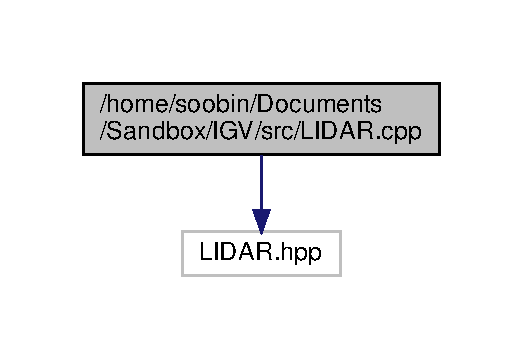
\includegraphics[width=251pt]{LIDAR_8cpp__incl}
\end{center}
\end{figure}

\hypertarget{LIDAR_8cpp_source}{}\section{L\+I\+D\+A\+R.\+cpp}
\label{LIDAR_8cpp_source}\index{/home/soobin/\+Documents/\+Sandbox/\+I\+G\+V/src/\+L\+I\+D\+A\+R.\+cpp@{/home/soobin/\+Documents/\+Sandbox/\+I\+G\+V/src/\+L\+I\+D\+A\+R.\+cpp}}

\begin{DoxyCode}
00001 \textcolor{preprocessor}{#}\textcolor{preprocessor}{include} \textcolor{preprocessor}{"LIDAR.hpp"}
00002 
00003 \textcolor{keyword}{using} \textcolor{keyword}{namespace} igv;
00004 
00005 \textcolor{preprocessor}{#}\textcolor{preprocessor}{ifndef} \textcolor{preprocessor}{SIMULATION}
00006 \textcolor{keyword}{using} \textcolor{keyword}{namespace} mn::CppLinuxSerial;
00007 
00008 LIDAR::LIDAR(): myport(LIDARPORT, B9600)\{\}
00009 
00010 \textcolor{keywordtype}{void} LIDAR::Probe()\{
00011 
00012 
00013 \}
00014 
00015 \textcolor{preprocessor}{#}\textcolor{preprocessor}{else}
00016 
00017 
00018 
00019 \textcolor{preprocessor}{#}\textcolor{preprocessor}{endif}
\end{DoxyCode}

\hypertarget{main_8cpp}{}\section{/home/soobin/\+Documents/\+Sandbox/\+I\+G\+V/src/main.cpp File Reference}
\label{main_8cpp}\index{/home/soobin/\+Documents/\+Sandbox/\+I\+G\+V/src/main.\+cpp@{/home/soobin/\+Documents/\+Sandbox/\+I\+G\+V/src/main.\+cpp}}
{\ttfamily \#include \char`\"{}I\+G\+V.\+hpp\char`\"{}}\newline
{\ttfamily \#include \char`\"{}test.\+hpp\char`\"{}}\newline
{\ttfamily \#include $<$string$>$}\newline
Include dependency graph for main.\+cpp\+:
\nopagebreak
\begin{figure}[H]
\begin{center}
\leavevmode
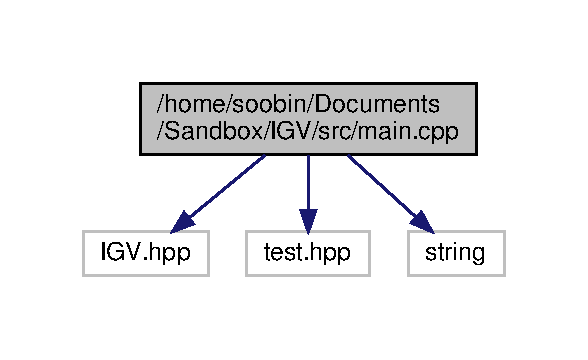
\includegraphics[width=282pt]{main_8cpp__incl}
\end{center}
\end{figure}
\subsection*{Functions}
\begin{DoxyCompactItemize}
\item 
int \hyperlink{main_8cpp_a3c04138a5bfe5d72780bb7e82a18e627}{main} (int argc, char $\ast$$\ast$argv)
\end{DoxyCompactItemize}


\subsection{Function Documentation}
\mbox{\Hypertarget{main_8cpp_a3c04138a5bfe5d72780bb7e82a18e627}\label{main_8cpp_a3c04138a5bfe5d72780bb7e82a18e627}} 
\index{main.\+cpp@{main.\+cpp}!main@{main}}
\index{main@{main}!main.\+cpp@{main.\+cpp}}
\subsubsection{\texorpdfstring{main()}{main()}}
{\footnotesize\ttfamily int main (\begin{DoxyParamCaption}\item[{int}]{argc,  }\item[{char $\ast$$\ast$}]{argv }\end{DoxyParamCaption})}



Definition at line \hyperlink{main_8cpp_source_l00010}{10} of file \hyperlink{main_8cpp_source}{main.\+cpp}.


\begin{DoxyCode}
00010                                \{
00011 
00012 \textcolor{preprocessor}{#ifdef DEBUG}
00013 
00014   \textcolor{keywordflow}{if}(argc > 1)\{
00015 
00016     \textcolor{keywordflow}{if}(!(\textcolor{keywordtype}{string}(argv[1])).compare(\textcolor{stringliteral}{"--setup"}))\{
00017 
00018       IGV \hyperlink{namespaceigv}{igv};
00019       igv.Setup();
00020 
00021     \}
00022 
00023     \textcolor{keywordflow}{else}\{
00024 
00025       cout << \textcolor{stringliteral}{"Testing Window"} << endl;
00026 
00027       Test test(\textcolor{stringliteral}{"../test/test.log"});
00028 
00029       \textcolor{keywordflow}{if}(argc > 2)\{
00030       
00031         \textcolor{keywordtype}{string} obj, filename;
00032 
00033         \textcolor{keywordflow}{for}(\textcolor{keywordtype}{int} i = 2; i < argc; i++)\{
00034         
00035           obj = argv[i];
00036         
00037           \textcolor{keywordflow}{if}(!obj.compare(\textcolor{stringliteral}{"all"}))           test.RunAllTests();
00038           \textcolor{keywordflow}{else} \textcolor{keywordflow}{if}(!obj.compare(\textcolor{stringliteral}{"cam"}))      test.CameraTest();
00039           \textcolor{keywordflow}{else} \textcolor{keywordflow}{if}(!obj.compare(\textcolor{stringliteral}{"motor"}))    test.MotorTest();
00040           \textcolor{keywordflow}{else} \textcolor{keywordflow}{if}(!obj.compare(\textcolor{stringliteral}{"od"}))       test.ObjectDetectionTest();
00041           \textcolor{keywordflow}{else} \textcolor{keywordflow}{if}(!obj.compare(\textcolor{stringliteral}{"ld"}))       test.LaneDetectionTest(\textcolor{stringliteral}{"../test/test.jpeg"});
00042           \textcolor{keywordflow}{else} \textcolor{keywordflow}{if}(!obj.compare(\textcolor{stringliteral}{"lidar"}))    test.LIDARTest();
00043           \textcolor{keywordflow}{else} \textcolor{keywordflow}{if}(!obj.compare(\textcolor{stringliteral}{"gps"}))      test.GPSTest();
00044           \textcolor{keywordflow}{else} cout << \textcolor{stringliteral}{"Invalid Option: "} << obj << endl;
00045       
00046         \} 
00047       \}
00048     \}
00049   \}
00050 
00051   \textcolor{keywordflow}{else} 
00052     cout  << \textcolor{stringliteral}{"Welcome to the IGV Help Menu\(\backslash\)n"}
00053           << \textcolor{stringliteral}{"'--test' Runs the Tests to specify which one put options after:\(\backslash\)n"}
00054           << \textcolor{stringliteral}{"\(\backslash\)t'cam', 'gps', 'all', 'motor', 'lidar', 'ld', 'od', 'sensors'\(\backslash\)n"};
00055 
00056     
00057   \textcolor{keywordflow}{return} EXIT\_SUCCESS;
00058   
00059 \textcolor{preprocessor}{#endif}
00060 
00061   IGV igv;
00062 
00063   igv.Setup();
00064   igv.Run();
00065 
00066 \}
\end{DoxyCode}

\hypertarget{main_8cpp_source}{}\section{main.\+cpp}
\label{main_8cpp_source}\index{/home/soobin/\+Documents/\+Sandbox/\+I\+G\+V/src/main.\+cpp@{/home/soobin/\+Documents/\+Sandbox/\+I\+G\+V/src/main.\+cpp}}

\begin{DoxyCode}
00001 
00002 \textcolor{preprocessor}{#}\textcolor{preprocessor}{include} \textcolor{preprocessor}{"IGV.hpp"}
00003 \textcolor{preprocessor}{#}\textcolor{preprocessor}{include} \textcolor{preprocessor}{"test.hpp"}
00004 \textcolor{preprocessor}{#}\textcolor{preprocessor}{include} \textcolor{preprocessor}{<}\textcolor{preprocessor}{string}\textcolor{preprocessor}{>}
00005 
00006 \textcolor{keyword}{using} \textcolor{keyword}{namespace} std;
00007 \textcolor{keyword}{using} \textcolor{keyword}{namespace} cv;
00008 \textcolor{keyword}{using} \textcolor{keyword}{namespace} igv;
00009 
\Hypertarget{main_8cpp_source_l00010}\hyperlink{main_8cpp_a3c04138a5bfe5d72780bb7e82a18e627}{00010} \textcolor{keywordtype}{int} \hyperlink{main_8cpp_a3c04138a5bfe5d72780bb7e82a18e627}{main}(\textcolor{keywordtype}{int} argc, \textcolor{keywordtype}{char}** argv)\{
00011 
00012 \textcolor{preprocessor}{#}\textcolor{preprocessor}{ifdef} \textcolor{preprocessor}{DEBUG}
00013 
00014   \textcolor{keywordflow}{if}(argc > 1)\{
00015 
00016     \textcolor{keywordflow}{if}(!(string(argv[1])).compare(\textcolor{stringliteral}{"--setup"}))\{
00017 
00018       IGV igv;
00019       igv.Setup();
00020 
00021     \}
00022 
00023     \textcolor{keywordflow}{else}\{
00024 
00025       cout << \textcolor{stringliteral}{"Testing Window"} << endl;
00026 
00027       Test test(\textcolor{stringliteral}{"../test/test.log"});
00028 
00029       \textcolor{keywordflow}{if}(argc > 2)\{
00030 
00031         string obj, filename;
00032 
00033         \textcolor{keywordflow}{for}(\textcolor{keywordtype}{int} i = 2; i < argc; i++)\{
00034 
00035           obj = argv[i];
00036 
00037           \textcolor{keywordflow}{if}(!obj.compare(\textcolor{stringliteral}{"all"}))           test.RunAllTests();
00038           \textcolor{keywordflow}{else} \textcolor{keywordflow}{if}(!obj.compare(\textcolor{stringliteral}{"cam"}))      test.CameraTest();
00039           \textcolor{keywordflow}{else} \textcolor{keywordflow}{if}(!obj.compare(\textcolor{stringliteral}{"motor"}))    test.MotorTest();
00040           \textcolor{keywordflow}{else} \textcolor{keywordflow}{if}(!obj.compare(\textcolor{stringliteral}{"od"}))       test.ObjectDetectionTest();
00041           \textcolor{keywordflow}{else} \textcolor{keywordflow}{if}(!obj.compare(\textcolor{stringliteral}{"ld"}))       test.LaneDetectionTest(\textcolor{stringliteral}{"../test/test.jpeg"});
00042           \textcolor{keywordflow}{else} \textcolor{keywordflow}{if}(!obj.compare(\textcolor{stringliteral}{"lidar"}))    test.LIDARTest();
00043           \textcolor{keywordflow}{else} \textcolor{keywordflow}{if}(!obj.compare(\textcolor{stringliteral}{"gps"}))      test.GPSTest();
00044           \textcolor{keywordflow}{else} cout << \textcolor{stringliteral}{"Invalid Option: "} << obj << endl;
00045 
00046         \}
00047       \}
00048     \}
00049   \}
00050 
00051   \textcolor{keywordflow}{else}
00052     cout  << \textcolor{stringliteral}{"Welcome to the IGV Help Menu\(\backslash\)n"}
00053           << \textcolor{stringliteral}{"'--test' Runs the Tests to specify which one put options after:\(\backslash\)n"}
00054           << \textcolor{stringliteral}{"\(\backslash\)t'cam', 'gps', 'all', 'motor', 'lidar', 'ld', 'od', 'sensors'\(\backslash\)n"};
00055 
00056 
00057   \textcolor{keywordflow}{return} EXIT\_SUCCESS;
00058 
00059 \textcolor{preprocessor}{#}\textcolor{preprocessor}{endif}
00060 
00061   IGV igv;
00062 
00063   igv.Setup();
00064   igv.Run();
00065 
00066 \}
\end{DoxyCode}

\hypertarget{ObjectDetection_8cpp}{}\section{/home/soobin/\+Documents/\+Sandbox/\+I\+G\+V/src/\+Object\+Detection.cpp File Reference}
\label{ObjectDetection_8cpp}\index{/home/soobin/\+Documents/\+Sandbox/\+I\+G\+V/src/\+Object\+Detection.\+cpp@{/home/soobin/\+Documents/\+Sandbox/\+I\+G\+V/src/\+Object\+Detection.\+cpp}}
{\ttfamily \#include \char`\"{}Object\+Detection.\+hpp\char`\"{}}\newline
Include dependency graph for Object\+Detection.\+cpp\+:
\nopagebreak
\begin{figure}[H]
\begin{center}
\leavevmode
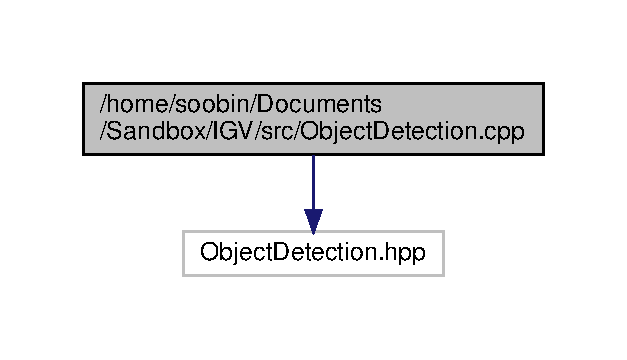
\includegraphics[width=301pt]{ObjectDetection_8cpp__incl}
\end{center}
\end{figure}

\hypertarget{ObjectDetection_8cpp_source}{}\section{Object\+Detection.\+cpp}
\label{ObjectDetection_8cpp_source}\index{/home/soobin/\+Documents/\+Sandbox/\+I\+G\+V/src/\+Object\+Detection.\+cpp@{/home/soobin/\+Documents/\+Sandbox/\+I\+G\+V/src/\+Object\+Detection.\+cpp}}

\begin{DoxyCode}
00001 
00002 \textcolor{preprocessor}{#}\textcolor{preprocessor}{include} \textcolor{preprocessor}{"ObjectDetection.hpp"}
00003 
00004 \textcolor{keyword}{using} \textcolor{keyword}{namespace} igv;
00005 
00006 \textcolor{comment}{// Stream operator allows the lanes to be printed to file of stdout}
00007 ostream& igv::operator<<(ostream& os, Object& obj)\{
00008 
00009     os << \textcolor{stringliteral}{"Object Type "} << obj.classification << endl;
00010     os << \textcolor{stringliteral}{"At Angle "} << obj.angle << endl;
00011     os << \textcolor{stringliteral}{"With Distance "} << obj.distance << endl;
00012 
00013     \textcolor{keywordflow}{return} os;
00014 \}
00015 
00016 \textcolor{preprocessor}{#}\textcolor{preprocessor}{ifndef} \textcolor{preprocessor}{CUDA}  \textcolor{comment}{// if not using the GPU}
00017 
00018 uint32\_t ObjDetector::DetectObjects(list<Object>& objects, Mat& image)\{
00019 
00020     \textcolor{keywordflow}{return} objects.size();
00021 
00022 \}
00023 
00024 uint32\_t ObjDetector::DetectObjects(Mat& Image)\{
00025 
00026     busy = \textcolor{keyword}{true};
00027 
00028     busy = \textcolor{keyword}{false};
00029 
00030     \textcolor{keywordflow}{return} \textcolor{keyword}{this}->objects.size();
00031 \}
00032 
00033 \textcolor{preprocessor}{#}\textcolor{preprocessor}{else}
00034 
00035 uint32\_t ObjDetector::DetectObjects(list<Object>& objs, Mat& Image)\{
00036 
00037     \textcolor{keywordflow}{return} objs.size();
00038 
00039 \}
00040 
00041 
00042 uint32\_t ObjDetector::DetectObjects(Mat& Image)\{
00043 
00044     busy = \textcolor{keyword}{true};
00045 
00046     busy = \textcolor{keyword}{false};
00047 
00048     \textcolor{keywordflow}{return} objs.size();
00049 
00050 \}
00051 
00052 \textcolor{preprocessor}{#}\textcolor{preprocessor}{endif}
\end{DoxyCode}

\hypertarget{Sensors_8cpp}{}\section{/home/soobin/\+Documents/\+Sandbox/\+I\+G\+V/src/\+Sensors.cpp File Reference}
\label{Sensors_8cpp}\index{/home/soobin/\+Documents/\+Sandbox/\+I\+G\+V/src/\+Sensors.\+cpp@{/home/soobin/\+Documents/\+Sandbox/\+I\+G\+V/src/\+Sensors.\+cpp}}
{\ttfamily \#include \char`\"{}Sensors.\+hpp\char`\"{}}\newline
Include dependency graph for Sensors.\+cpp\+:
\nopagebreak
\begin{figure}[H]
\begin{center}
\leavevmode
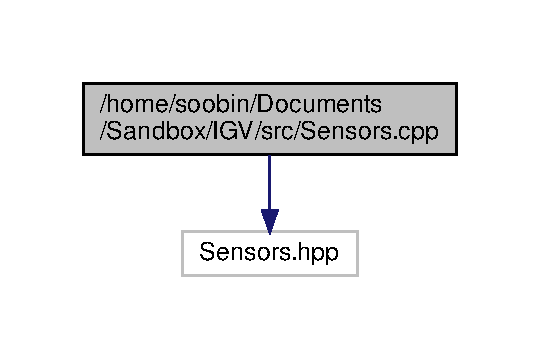
\includegraphics[width=259pt]{Sensors_8cpp__incl}
\end{center}
\end{figure}

\hypertarget{Sensors_8cpp_source}{}\section{Sensors.\+cpp}
\label{Sensors_8cpp_source}\index{/home/soobin/\+Documents/\+Sandbox/\+I\+G\+V/src/\+Sensors.\+cpp@{/home/soobin/\+Documents/\+Sandbox/\+I\+G\+V/src/\+Sensors.\+cpp}}

\begin{DoxyCode}
00001 \textcolor{preprocessor}{#}\textcolor{preprocessor}{include} \textcolor{preprocessor}{"Sensors.hpp"}
00002 
00003 \textcolor{preprocessor}{#}\textcolor{preprocessor}{ifndef} \textcolor{preprocessor}{SIMULATION}
00004 \textcolor{keyword}{using} \textcolor{keyword}{namespace} mn::CppLinuxSerial;
00005 \textcolor{keyword}{using} \textcolor{keyword}{namespace} igv;
00006 
00007 \textcolor{keywordtype}{void} Magno::Probe()\{
00008 
00009 \}
00010 
00011 
00012 UltraSonic::UltraSonic()\{
00013 
00014     GPIO::setmode(GPIO::BOARD);
00015 
00016     GPIO::setup(ULTRA\_IN, GPIO::IN);
00017     GPIO::setup(ULTRA\_OUT, GPIO::OUT, GPIO::LOW);
00018 
00019 \}
00020 
00021 \textcolor{keywordtype}{void} UltraSonic::Probe() \{
00022 
00023     busy = \textcolor{keyword}{true};
00024 
00025     GPIO::output(ULTRA\_OUT, GPIO::HIGH);  \textcolor{comment}{// trigger a pulse}
00026     \textcolor{keyword}{auto} start = std::chrono::system\_clock::now();  \textcolor{comment}{// get the current time}
00027     \textcolor{keywordflow}{while}(!GPIO::input(ULTRA\_IN));  \textcolor{comment}{// wait for a signal on the input line}
00028     \textcolor{keyword}{auto} end = std::chrono::system\_clock::now();  \textcolor{comment}{// get the current time}
00029 
00030     std::chrono::duration<\textcolor{keywordtype}{double}> timediff = end - start; \textcolor{comment}{// calculate the difference}
00031 
00032     \textcolor{keyword}{this}->distance = VSOUND\_D2*timediff.count(); \textcolor{comment}{// v = d/t -> d = v*t: t = timediff/2, v = speed of
       sound}
00033     GPIO::output(ULTRA\_OUT, GPIO::LOW);  \textcolor{comment}{// reset}
00034 
00035     busy = \textcolor{keyword}{false};
00036 
00037 \}
00038 
00039 
00040 \textcolor{preprocessor}{#}\textcolor{preprocessor}{else}
00041 
00042 
00043 \textcolor{preprocessor}{#}\textcolor{preprocessor}{endif}
\end{DoxyCode}

\hypertarget{test_8cpp}{}\section{/home/soobin/\+Documents/\+Sandbox/\+I\+G\+V/test/test.cpp File Reference}
\label{test_8cpp}\index{/home/soobin/\+Documents/\+Sandbox/\+I\+G\+V/test/test.\+cpp@{/home/soobin/\+Documents/\+Sandbox/\+I\+G\+V/test/test.\+cpp}}
{\ttfamily \#include \char`\"{}test.\+hpp\char`\"{}}\newline
Include dependency graph for test.\+cpp\+:
\nopagebreak
\begin{figure}[H]
\begin{center}
\leavevmode
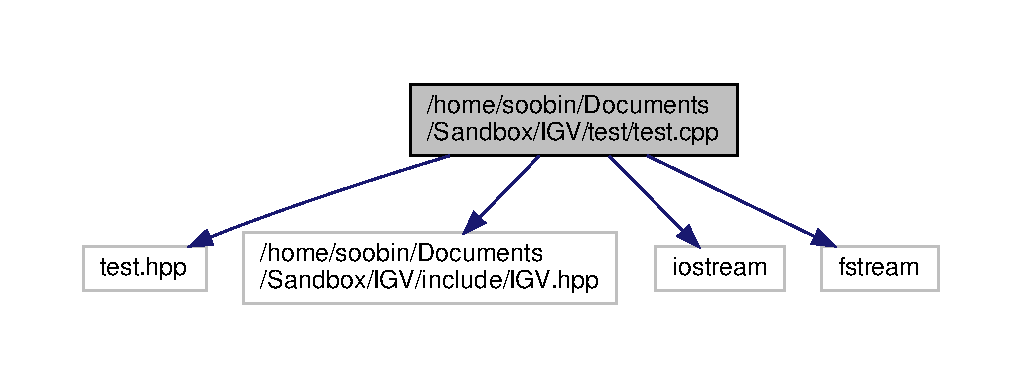
\includegraphics[width=350pt]{test_8cpp__incl}
\end{center}
\end{figure}

\hypertarget{test_8cpp_source}{}\section{test.\+cpp}
\label{test_8cpp_source}\index{/home/soobin/\+Documents/\+Sandbox/\+I\+G\+V/test/test.\+cpp@{/home/soobin/\+Documents/\+Sandbox/\+I\+G\+V/test/test.\+cpp}}

\begin{DoxyCode}
00001 
00002 \textcolor{preprocessor}{#}\textcolor{preprocessor}{include} \textcolor{preprocessor}{"test.hpp"}
00003 
00004 \textcolor{keyword}{using} \textcolor{keyword}{namespace} std;
00005 \textcolor{keyword}{using} \textcolor{keyword}{namespace} cv;
00006 \textcolor{keyword}{using} \textcolor{keyword}{namespace} igv;
00007 
00008 Test::Test(\textcolor{keyword}{const} \textcolor{keywordtype}{char} *logfile) : logfile(logfile) \{\}
00009 
00010 Test::~Test() \{ logfile.close(); \}
00011 
00012 \textcolor{keywordtype}{bool} Test::CameraTest()
00013 \{
00014 
00015   \textcolor{keywordtype}{bool} Passed = \textcolor{keyword}{true};
00016 
00017   logfile << \textcolor{stringliteral}{"Creating Lane Camera Object \(\backslash\)n"};
00018   Camera cam1(LANECAMPORT);
00019 
00020   logfile << \textcolor{stringliteral}{"Taking a Picture \(\backslash\)n"};
00021   cam1.Capture();
00022 
00023   logfile << \textcolor{stringliteral}{"Retrieving the Image \(\backslash\)n"};
00024   Mat testimage = cam1.GetImage();
00025 
00026   logfile << \textcolor{stringliteral}{"Image Specs: \(\backslash\)n"}
00027           << \textcolor{stringliteral}{"========================="}
00028           << \textcolor{stringliteral}{"Is Empty:       "} << testimage.empty() << endl
00029           << \textcolor{stringliteral}{"Dimensionality: "} << testimage.dims << endl
00030           << \textcolor{stringliteral}{"Pixel Format:   "} << testimage.depth() << endl
00031           << \textcolor{stringliteral}{"Size:           "} << testimage.size << endl
00032           << endl;
00033 
00034   \textcolor{keywordflow}{if} (testimage.empty() || !testimage.size)
00035     Passed = \textcolor{keyword}{false};
00036   \textcolor{keywordflow}{else}
00037     Passed = \textcolor{keyword}{true};
00038 
00039   logfile << \textcolor{stringliteral}{"Creating Object Camera Object \(\backslash\)n"};
00040   Camera cam2(OBJCAMPORT);
00041 
00042   logfile << \textcolor{stringliteral}{"Taking a Picture: \(\backslash\)n"};
00043   cam2.Capture();
00044 
00045   logfile << \textcolor{stringliteral}{"Retrieving the Image \(\backslash\)n"};
00046   logfile << \textcolor{stringliteral}{"Image Specs: \(\backslash\)n"}
00047           << \textcolor{stringliteral}{"========================="}
00048           << \textcolor{stringliteral}{"Is Empty:       "} << testimage.empty() << endl
00049           << \textcolor{stringliteral}{"Dimensionality: "} << testimage.dims << endl
00050           << \textcolor{stringliteral}{"Pixel Format:   "} << testimage.depth() << endl
00051           << \textcolor{stringliteral}{"Size:           "} << testimage.size << endl
00052           << endl
00053           << endl;
00054 
00055   \textcolor{keywordflow}{if} (testimage.empty() || !testimage.size)
00056     Passed = \textcolor{keyword}{false};
00057   \textcolor{keywordflow}{else}
00058     Passed = \textcolor{keyword}{true};
00059 
00060   \textcolor{keywordflow}{return} Passed;
00061 \}
00062 
00063 \textcolor{keywordtype}{bool} Test::LaneDetectionTest(string filename)
00064 \{
00065 
00066   \textcolor{keywordtype}{bool} passed = \textcolor{keyword}{true};
00067 
00068   LaneDetector ld;
00069 
00070   logfile << \textcolor{stringliteral}{"Opening Image: << filename << endl"};
00071   Mat testmat = imread(filename); \textcolor{comment}{// load the sample image to test and compare}
00072 
00073   logfile << \textcolor{stringliteral}{"Retrieving the Image \(\backslash\)n"};
00074   logfile << \textcolor{stringliteral}{"Image Specs: \(\backslash\)n"}
00075           << \textcolor{stringliteral}{"========================="} << endl
00076           << \textcolor{stringliteral}{"Is Empty:       "} << testmat.empty() << endl
00077           << \textcolor{stringliteral}{"Dimensionality: "} << testmat.dims << endl
00078           << \textcolor{stringliteral}{"Pixel Format:   "} << testmat.depth() << endl
00079           << \textcolor{stringliteral}{"Size:           "} << testmat.size << endl << endl;
00080 
00081   \textcolor{keywordflow}{if} (!testmat.size || testmat.empty())
00082     passed = \textcolor{keyword}{false};
00083 
00084   logfile << \textcolor{stringliteral}{"Creating Empty Lane Array: Lanes Full of Zeros \(\backslash\)n"};
00085   array<Lane, 4> testlanes = \{Lane(\{0, 0\}), Lane(\{0, 0\})\};
00086 
00087   logfile << \textcolor{stringliteral}{"Detecting Lanes: \(\backslash\)n"};
00088 
00089   uint32\_t numlanes = LaneDetector::DetectLanes(testlanes, testmat);
00090   ld.DetectLanes(testmat);
00091 
00092   logfile << \textcolor{stringliteral}{"Printing Lanes: \(\backslash\)n"};
00093   logfile << \textcolor{stringliteral}{"Total Lanes Found: Static Call: "} << numlanes
00094           << \textcolor{stringliteral}{" Object Call: "} << ld.GetNumLanes() << endl;
00095 
00096   logfile << \textcolor{stringliteral}{"Static Lanes: "} << endl;
00097   \textcolor{keywordflow}{for} (Lane lane : testlanes)
00098     logfile << lane;
00099 
00100   logfile << \textcolor{stringliteral}{"Object Lanes: "} << endl;
00101   \textcolor{keywordflow}{for} (Lane lane : ld.GetLanes())
00102     logfile << lane;
00103 
00104   \textcolor{keywordflow}{return} passed;
00105 \}
00106 
00107 \textcolor{keywordtype}{bool} Test::LIDARTest() \{ \textcolor{keywordflow}{return} \textcolor{keyword}{true}; \}
00108 
00109 \textcolor{keywordtype}{bool} Test::GPSTest() \{ \textcolor{keywordflow}{return} \textcolor{keyword}{true}; \}
00110 
00111 \textcolor{keywordtype}{bool} Test::SensorsTest() \{ \textcolor{keywordflow}{return} \textcolor{keyword}{true}; \}
00112 
00113 \textcolor{keywordtype}{bool} Test::MotorTest() \{ \textcolor{keywordflow}{return} \textcolor{keyword}{true}; \}
00114 
00115 \textcolor{keywordtype}{bool} Test::ObjectDetectionTest() \{ \textcolor{keywordflow}{return} \textcolor{keyword}{true}; \}
00116 
00117 \textcolor{keywordtype}{bool} Test::RunAllTests()
00118 \{
00119 
00120   \textcolor{keywordtype}{bool} senstest = SensorsTest();
00121   \textcolor{keywordtype}{bool} motortest = MotorTest();
00122   \textcolor{keywordtype}{bool} ldtest = LaneDetectionTest(\textcolor{stringliteral}{"../test/test.jpeg"});
00123   \textcolor{keywordtype}{bool} odtest = ObjectDetectionTest();
00124   \textcolor{keywordtype}{bool} gpstest = GPSTest();
00125   \textcolor{keywordtype}{bool} lidartest = LIDARTest();
00126   \textcolor{keywordtype}{bool} camtest = CameraTest();
00127 
00128   cout << \textcolor{stringliteral}{"Sensor Test: "} << ((senstest) ? \textcolor{stringliteral}{"PASSED\(\backslash\)n"} : \textcolor{stringliteral}{"FAILED\(\backslash\)n"});
00129   cout << \textcolor{stringliteral}{"Camera Test: "} << ((camtest) ? \textcolor{stringliteral}{"PASSED\(\backslash\)n"} : \textcolor{stringliteral}{"FAILED\(\backslash\)n"});
00130   cout << \textcolor{stringliteral}{"Motor Test: "} << ((motortest) ? \textcolor{stringliteral}{"PASSED\(\backslash\)n"} : \textcolor{stringliteral}{"FAILED\(\backslash\)n"});
00131   cout << \textcolor{stringliteral}{"GPS Test: "} << ((gpstest) ? \textcolor{stringliteral}{"PASSED\(\backslash\)n"} : \textcolor{stringliteral}{"FAILED\(\backslash\)n"});
00132   cout << \textcolor{stringliteral}{"LIDAR Test: "} << ((lidartest) ? \textcolor{stringliteral}{"PASSED\(\backslash\)n"} : \textcolor{stringliteral}{"FAILED\(\backslash\)n"});
00133   cout << \textcolor{stringliteral}{"Lane Detection Test: "} << ((ldtest) ? \textcolor{stringliteral}{"PASSED\(\backslash\)n"} : \textcolor{stringliteral}{"FAILED\(\backslash\)n"});
00134   cout << \textcolor{stringliteral}{"Object Detection Test: "} << ((odtest) ? \textcolor{stringliteral}{"PASSED\(\backslash\)n"} : \textcolor{stringliteral}{"FAILED\(\backslash\)n"});
00135 
00136   \textcolor{keywordflow}{return} senstest && odtest && ldtest && motortest &&
00137          gpstest && lidartest && camtest;
00138 \}
\end{DoxyCode}

%--- End generated contents ---

% Index
\backmatter
\newpage
\phantomsection
\clearemptydoublepage
\addcontentsline{toc}{chapter}{Index}
\printindex

\end{document}
